\chapter{Problem Analysis}
Imagine sitting at a restaurant, eating a dinner and you notice a song that is playing, but you do not know which song it is. To figure out which song it is, there are various options. One of the options is to ask the staff which song it is. This solution may be fast but a little tedious. Another option is to go through all the songs in a music app, this solution is not the most effective way, though it spares you from an unwanted conversation. With modern technology you are able to download apps such as Shazam, which takes the good parts of both possibilities, you get spared from an unwanted conversation and it is quite fast.\\

\noindent This project describes a method of audio recognition. One way to recognise audio is to generate an audio fingerprint. In essence, audio fingerprinting is a method of determining unique characteristics in audio such as music. The generated audio fingerprint of a song will be stored in a database. An algorithm can then compare and match a recorded audio signal to the most alike audio fingerprint of a song in the database.\\ %(Denne linje skal måske slettes) In the following section two use cases of audio recognition are given. 
%Hvis den skal længere ned, er der brug for omskrivning i afsnittene, da vi ellers ikke for præsenteret audio fingerprint
\indent Shazam is an app with the purpose of recognising songs from a recording. The app is able to recognise a song even if ambient noise is present, such as in a restaurant or a car. When Shazam recognises a song, it gives the user the title of the track, the artist and the ability to stream the song on multiple different music platforms. \cite{ShazamDescription} \\
\indent Another use case for recognising audio fingerprints is identification of copyrighted materials. This can be useful for social media where users can upload material freely, since the social media will be economically responsible if copyrighted material is shared on their platform. This use case comes with several challenges. For instance, the audio can be compressed. The end user may not hear the difference between the compressed audio and the original recording, but it is still covered by copyright. Furthermore, the users may try to avoid identification systems by adding inaudible noise. \cite{haitsma2003highly}\\
\indent In both use cases, audio fingerprinting is useful when recognising music, because it is unnecessary to record the full length of a song to find enough unique characteristics. Therefore, it is possible to use the characteristics of a small portion of a song to compare the database to. 
The usefulness of audio fingerprinting is also apparent when there is noise on the recorded audio signal. An algorithm, that matches the most alike audio samples, can recognise songs through the noise, because of the unique characteristics of the audio fingerprints. 


\section{Problems and Parameters with Audio Recognition}
In the following, different aspects of audio recognition are analysed to get an overview of the challenges involved in creating an audio recognition system.\\
\indent To generate an audio fingerprint one might look at the semantics of a song such as genre and composition. Genres are generally difficult to quantify since they change as cultures change and sometimes overlap. Furthermore, there are almost endless ways to compose a song, it is therefore difficult to quantify. Therefore it is not feasible to generate an audio fingerprint using semantics. \cite{haitsma2003highly}\\
Another approach to generate an audio fingerprint for a piece of music, is to consider what songs and music consist of, and what sound really is.
Sound is created because of vibrations causing displacements and oscillations of molecules in a medium such as air, which can be considered as sound waves. The sound waves can be intercepted by the human ear, which can intercept frequencies between 20Hz and 20kHz. Therefore when working with music, it is only relevant to work within this spectrum. \cite[21]{Meinard2015Fundamentals}\\

When recording audio with a microphone, the audio signal becomes an electrical signal. The signal is represented as amplitude over time. Playing the tone of C\textsubscript{4} on a piano, the signal would be as shown in \autoref{fig:toneC4time}. Only considering the signal in the time domain, it can be difficult to find patterns in an recorded audio signal. 

\begin{figure}[H]
    \centering
    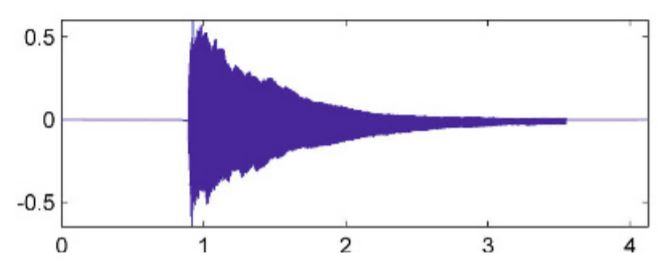
\includegraphics[width=0.8\textwidth]{figures/toneC4time.JPG}
    \caption{The tone C\textsubscript{4} played on a piano, in the time domain (vi replikerer selv denne figur.)}
    \label{fig:toneC4time}
\end{figure}

Instead of considering the electrical signal in the time domain, it might be preferable to consider the magnitude represented in the frequency domain. This can be done by using the Discrete Fourier Transform (DFT), which transforms, for instance, an electrical signal in the time domain, shown in \autoref{fig:toneC4time} to the complex frequency domain, shown in \autoref{fig:toneC4freq}.

This is beneficial because each tone consist of defined frequencies. For instance the tone C\textsubscript{4} played on a piano corresponds to the fundamental frequency of $261.6 \si{Hz}$ seen as the first peak in \autoref{fig:toneC4freq} \cite[29]{Meinard2015Fundamentals}. A tone consist of not only the fundamental frequency, but other frequencies called overtones. A general term for all the frequency peaks for a tone is called partial tones. The fundamental frequency is the first partial tone and the number of overtones in a tone can be described as $N-1$, where $N$ is the number of partial tones in a specific tone. For C\textsubscript{4} there are three partial tones, hence two overtones at approximately $523 \si{Hz}$ and $ 785 \si{Hz}$. \cite[41]{Meinard2015Fundamentals}
\begin{figure}[H]
    \centering
    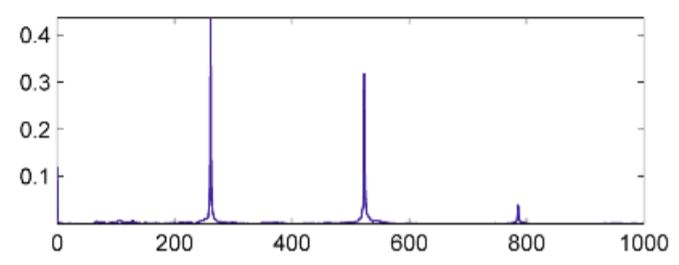
\includegraphics[width=0.8\textwidth]{figures/toneC4freq.JPG}
    \caption{Fourier transform of the audio recording of the tone C\textsubscript{4} played on a piano (vi replikerer selv denne figur.)}
    \label{fig:toneC4freq}
\end{figure}
Using the fact that tones have a fundamental frequency and overtones, it is possible to consider partial tones at a given time, in an audio recording, as unique characteristics in a song. When recording audio it is relevant to look into noise handling. Noise is often one of the factors which can cause the audio fingerprint to differ from the fingerprint in the database and therefore it might not be possible to recognise the song.\\
As described it is often desirable to recognise songs even if the input is noisy or distorted. The noise involved can be people speaking in the background, road noise in a car. The distortion could come from the speaker and amplifier the music is playing out of or from the sound bouncing around the room. To remove these unwanted aspects, it is necessary to filter the input.\cite{haitsma2003highly}\\

When a recorded song is filtered and the fingerprint is generated, it then needs to be matched with a song in the database. The database can potentially consist of millions of fingerprints. When the database is that large it is not effective to brute force a match, therefore an optimized search algorithm can be necessary. \cite{haitsma2003highly}

\section{Problem Definition}
Dette afsnit skal indeholde
\begin{itemize}
    \item System overview (blokdiagram)
    \item Vores fokus i projektet
    \item Hvorfor har vi valgt dette fokus
    \item Indsnæving til problemformulering
    \item Hvilke teorier vi vil anvende
    \item Et kort resumé af hvad der er blevet præsenteret i problemanalysen. 
\end{itemize}
\subsection{Audio Fingerprinting Process}
An audio fingerprinting system can generally be split into five parts.
\begin{itemize}
    \item \textbf{Audio recording:} Where the audio is digitised.
    \item \textbf{Filtering:} Removes the unwanted information of the recorded signal.
    \item \textbf{Generate fingerprint:} Generates the fingerprint needed to recognise the song.
    \item \textbf{Compare fingerprint to a database:} The generated fingerprint is compared to the fingerprints in the database.
    \item \textbf{Present the track information:} When the fingerprint is matched the relevant information is presented to the user.
\end{itemize}
This is illustrated in \autoref{fig:Fingerprint_process}.
These parts will be further explained in the next few sections.
   
\begin{figure} [H]
    \centering
    \begin{tikzpicture}[node distance = 4cm]
        \tikzstyle{box} = [rectangle, minimum width=3cm, minimum height=1cm, text centered, text width=3cm, draw=black]
        \tikzstyle{line} = [draw, -latex']
        \node (sampling) [box] {Audio recording};
        \node (filtering) [box, right of=sampling] {Filtering};
        \node (fingerprint) [box, right of=filtering] {Generate fingerprint};
        \node (compare) [box, below of=filtering, node distance =3cm] {Compare fingerprint to a database};
        \node (TrackInfo) [box, below of=sampling, node distance =3cm] {Present the track information};
        
        \path [line] (sampling) -- (filtering);
         \path [line] (filtering) -- (fingerprint);
        \path [line] (fingerprint) |- (compare);
         \path [line] (compare) -- (TrackInfo);
     \end{tikzpicture}
    \caption{The process of which an audio fingerprinting system uses audio recordings, filters the recordings, generates audio fingerprints, matches fingerprints and presents the user with the information.}
    \label{fig:Fingerprint_process}
\end{figure}


\section{Problem Statement}
How can an audio fingerprinting algorithm be constructed and recognise audio input even with noise and distortion? 

